\documentclass[11pt]{article}
\usepackage[utf8]{inputenc}
\usepackage{amsmath, amssymb}
\usepackage{graphicx}
\usepackage{hyperref}
\usepackage{geometry}
\usepackage{cite}
\usepackage{listings}
\usepackage{subcaption}

% Geometry settings
\geometry{a4paper, margin=1in}

% Title and author
\title{Planar Cable-Driven Robot}
\author{Arzaq Khan \\
Hamdan Raashid \\
}
\date{\today}

% Code block settings
\lstset{
  basicstyle=\ttfamily\small,
  breaklines=true,
  frame=single,
  numbers=left,
  numberstyle=\tiny,
  xleftmargin=2em,
  language=Python % Change as needed
}

\begin{document}

\maketitle


\section{Introduction}


\subsection{Project Description}
Our project is a planar cable-driven driven that continously tracks and follows objects in real time. If we had been able to
implement everything according to our initial plan, we would have been able to apply the robot in a logistics setting to pick and
place objects. Unfortunately, due to certain problems we encountered, which is discussed in a later section, we were unable to
strictly follow our original plans.

During the planning stage, we aimed to design a planar cable-driven robot that would pick a user selected target and drop off that
target to a user selected location. The user would first select the target in a video feed provided by a staionary camera and the
robot would move the end-effector to where the target is located. Next, a command would be given to the end-effector to switch on the
electromagnet to pick up the target. Then, the user would provide a location to drop off the target using
the same video feed and the robot would drop off the target at said location. 
Although our actual robot is similar to what we had planned initially, there are slight differences.

The main difference between what we built and we had planned lies in the parts we used and the end-effector. We had
planned to use an ESP32, a microcontroller, for its Bluetooth and WiFi features and stepper motors due to their precision.
Unfortunately, we could not get the stepper motors to work. We initially figured that it was a power issue, but even
after connecting the motors to an external power supply, we could not get the motors to move. As for the end-effector,
we could not mount an electromagnet on it due to issues discussed in a subsequent section. To summarize, what we have
is a robot that can continously track and follow objects, but cannot pick them up.

\begin{figure}[h!]
\centering

\begin{subfigure}[b]{0.3\textwidth}
    \centering
    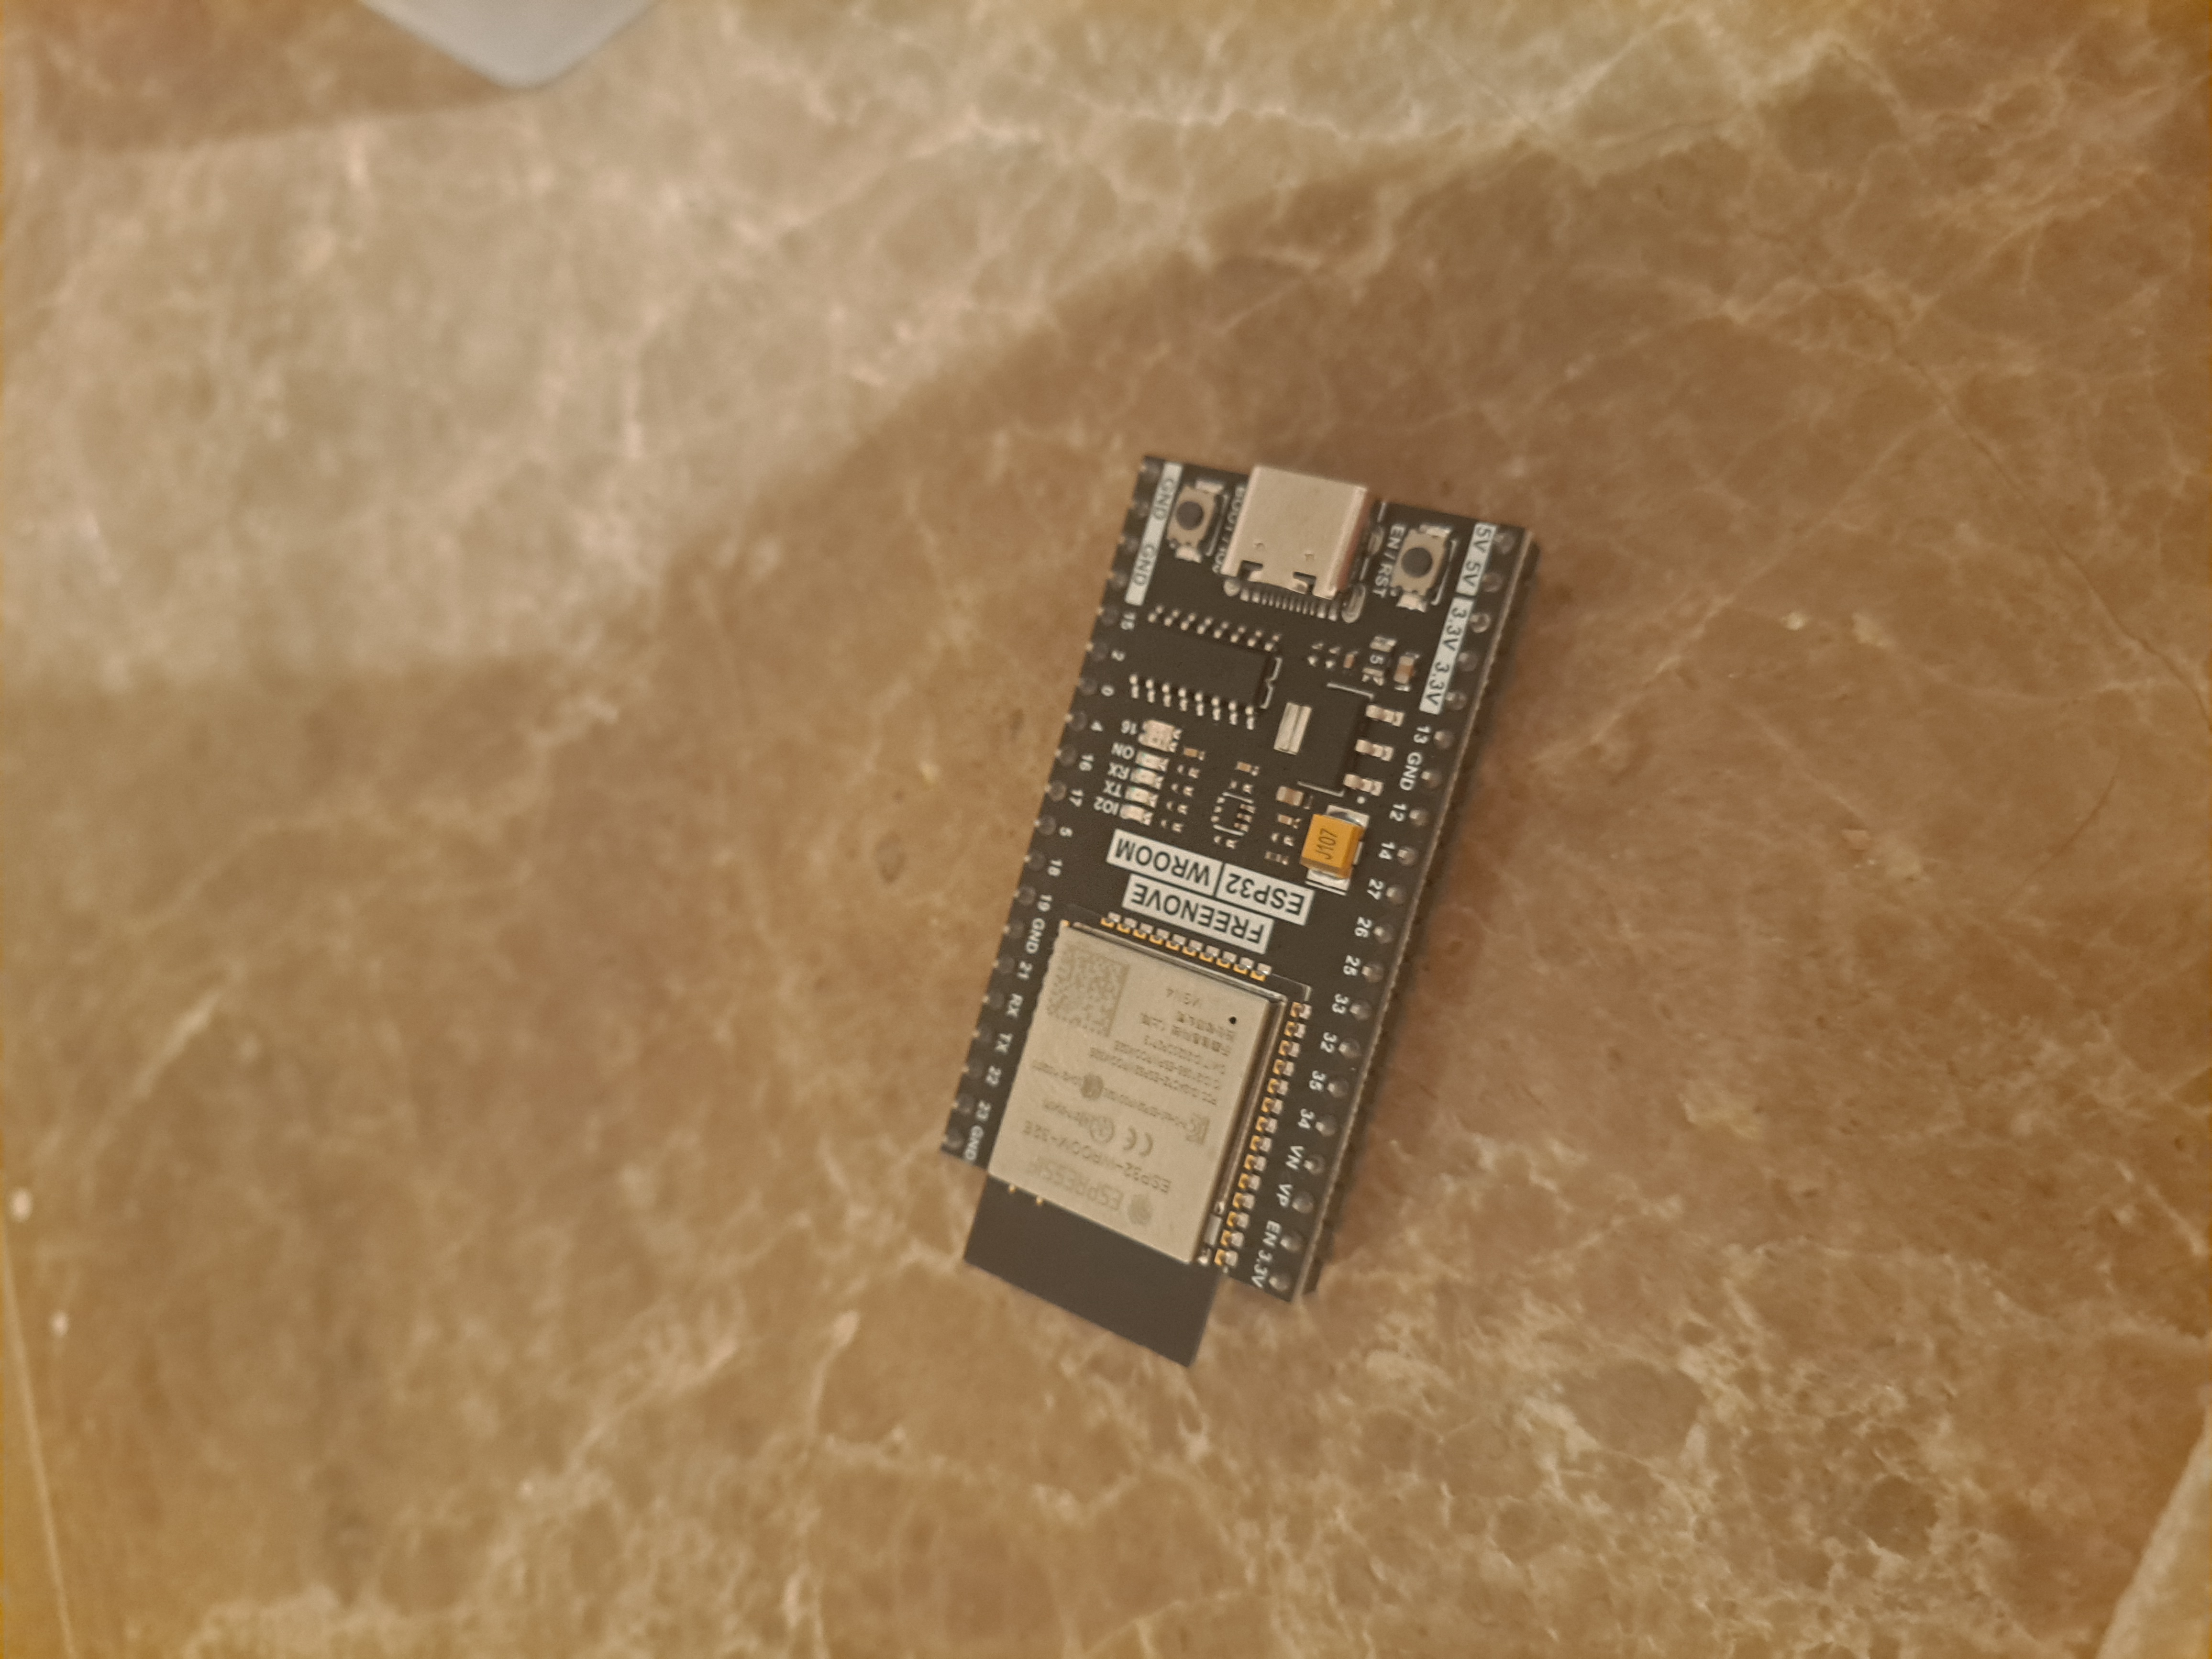
\includegraphics[width=\textwidth]{ESP32Img.jpg}
    \caption{An ESP32 microcontroller.}
    \label{fig:figure1}
\end{subfigure}
\hfill
\begin{subfigure}[b]{0.3\textwidth}
    \centering
    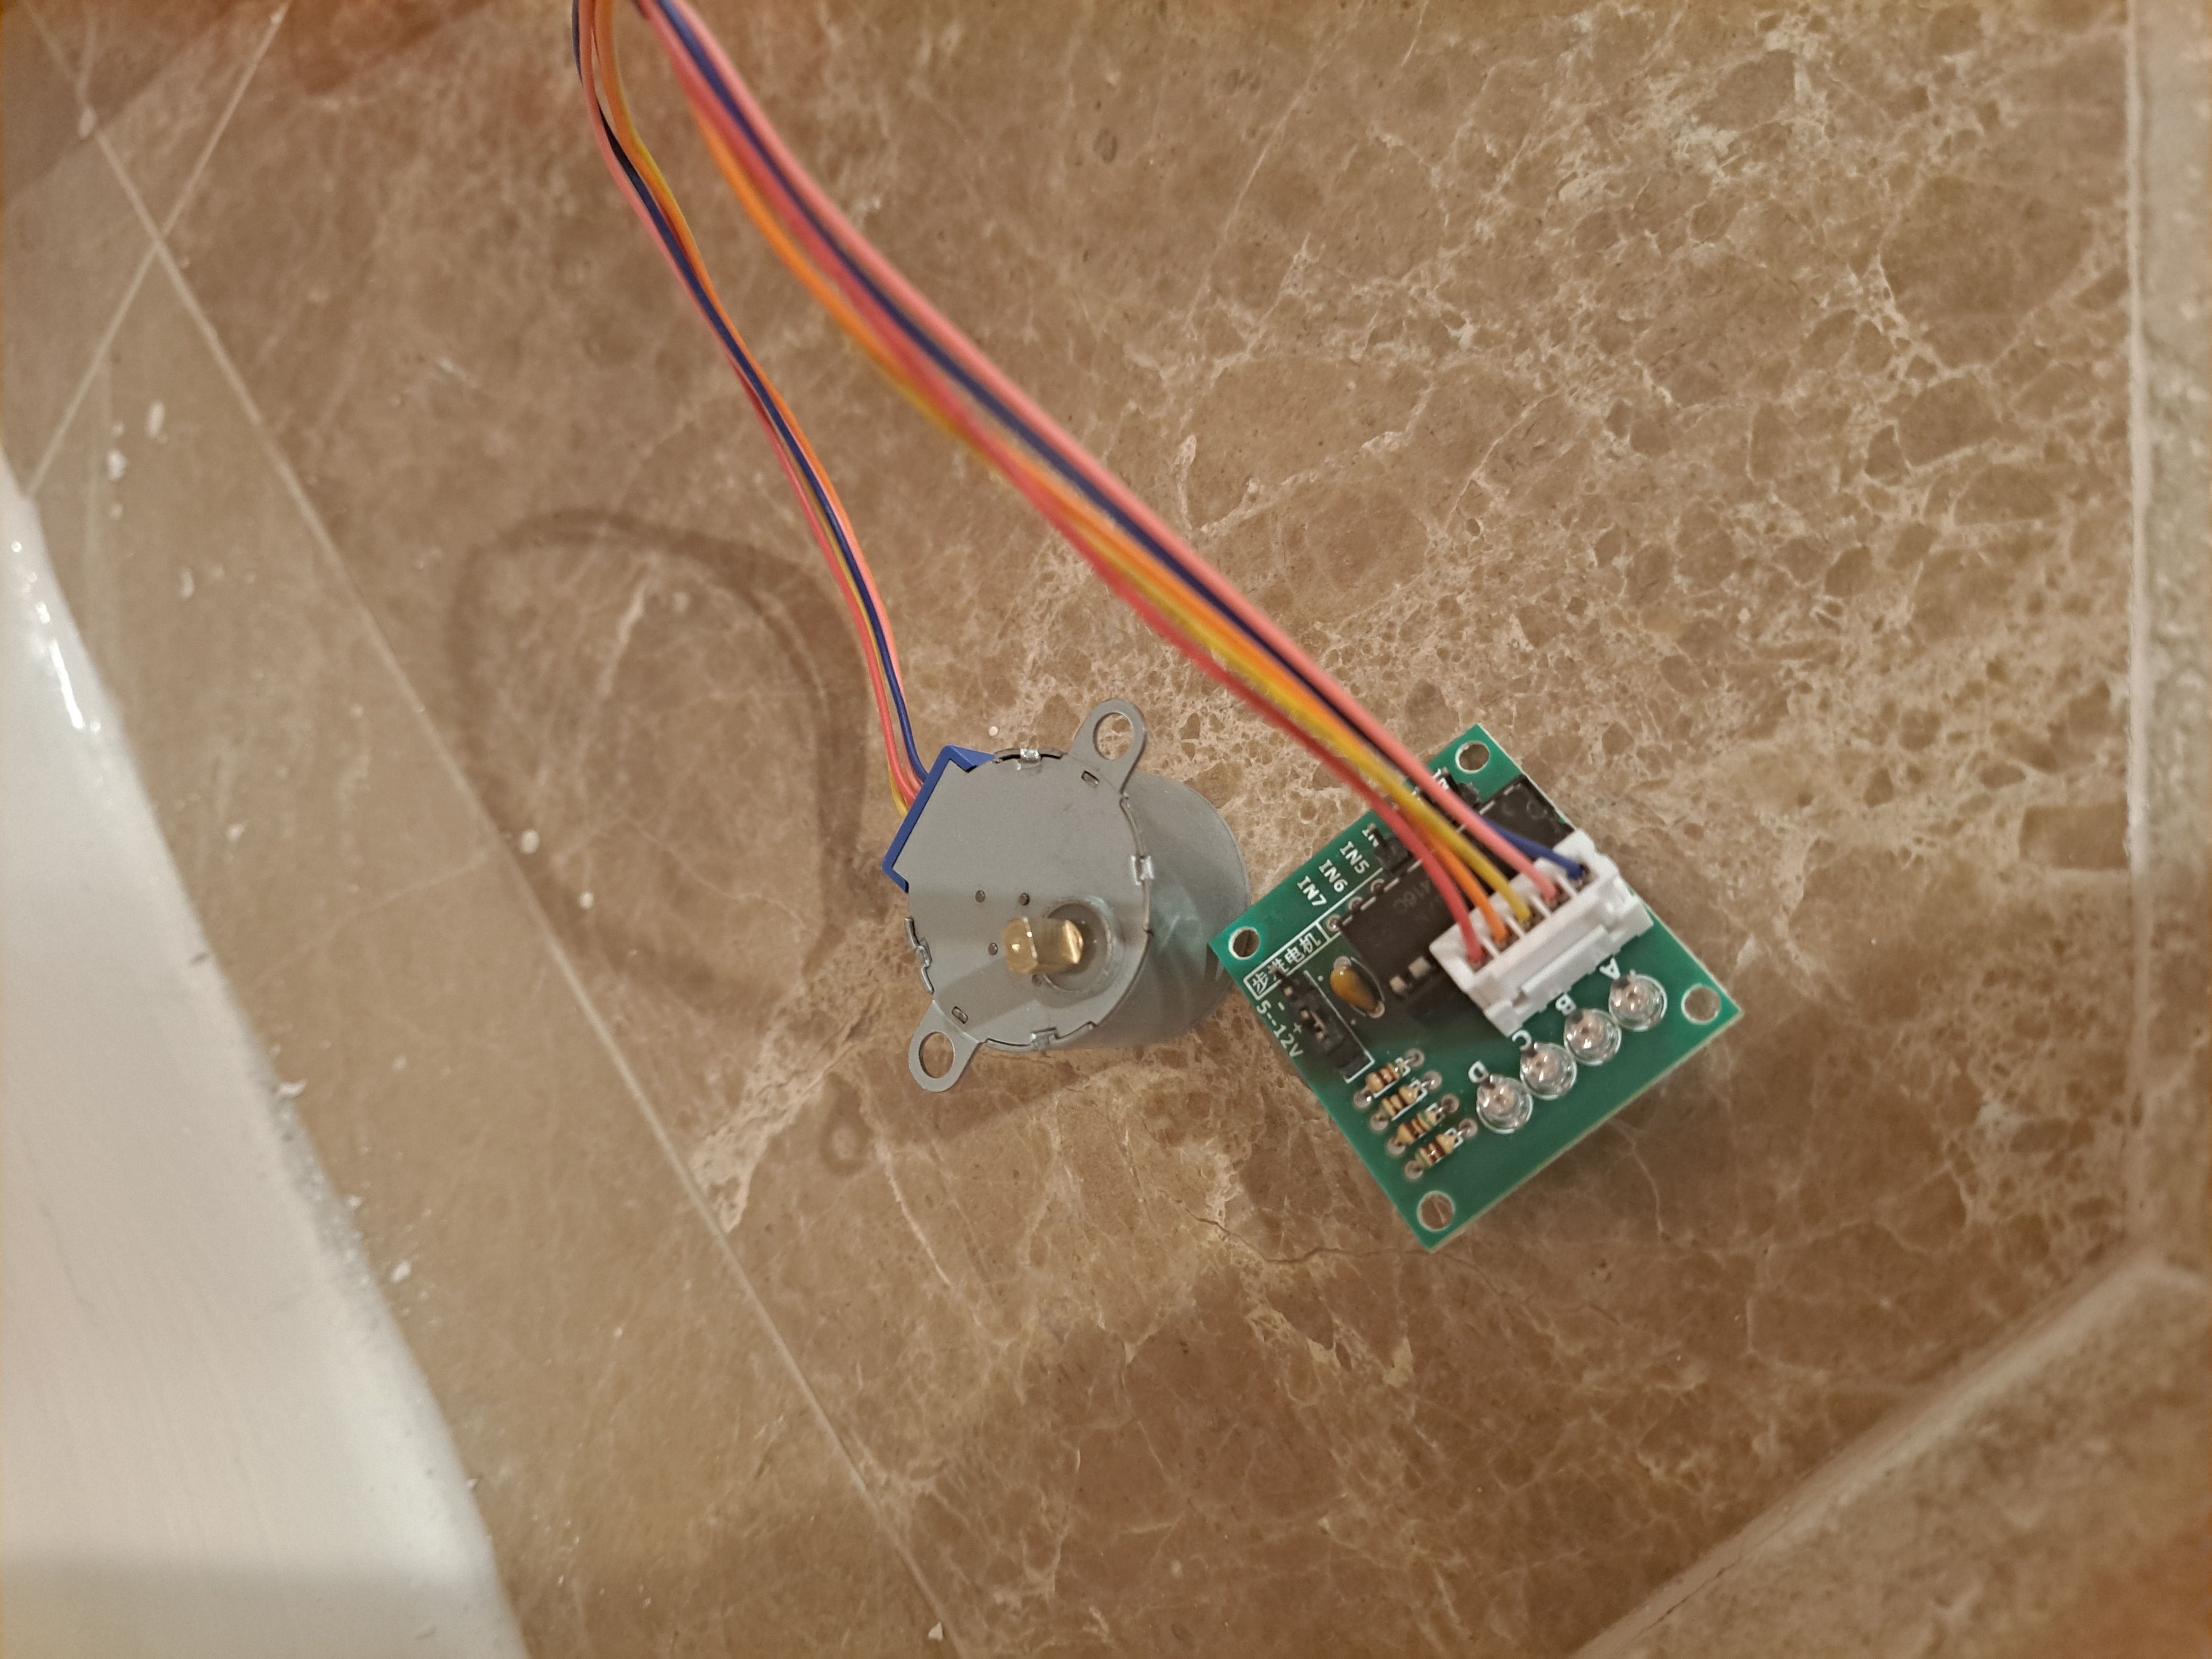
\includegraphics[width=\textwidth]{MotorImg.jpg}
    \caption{A stepper motor.}
    \label{fig:figure2}
\end{subfigure}
\hfill
\begin{subfigure}[b]{0.3\textwidth}
    \centering
    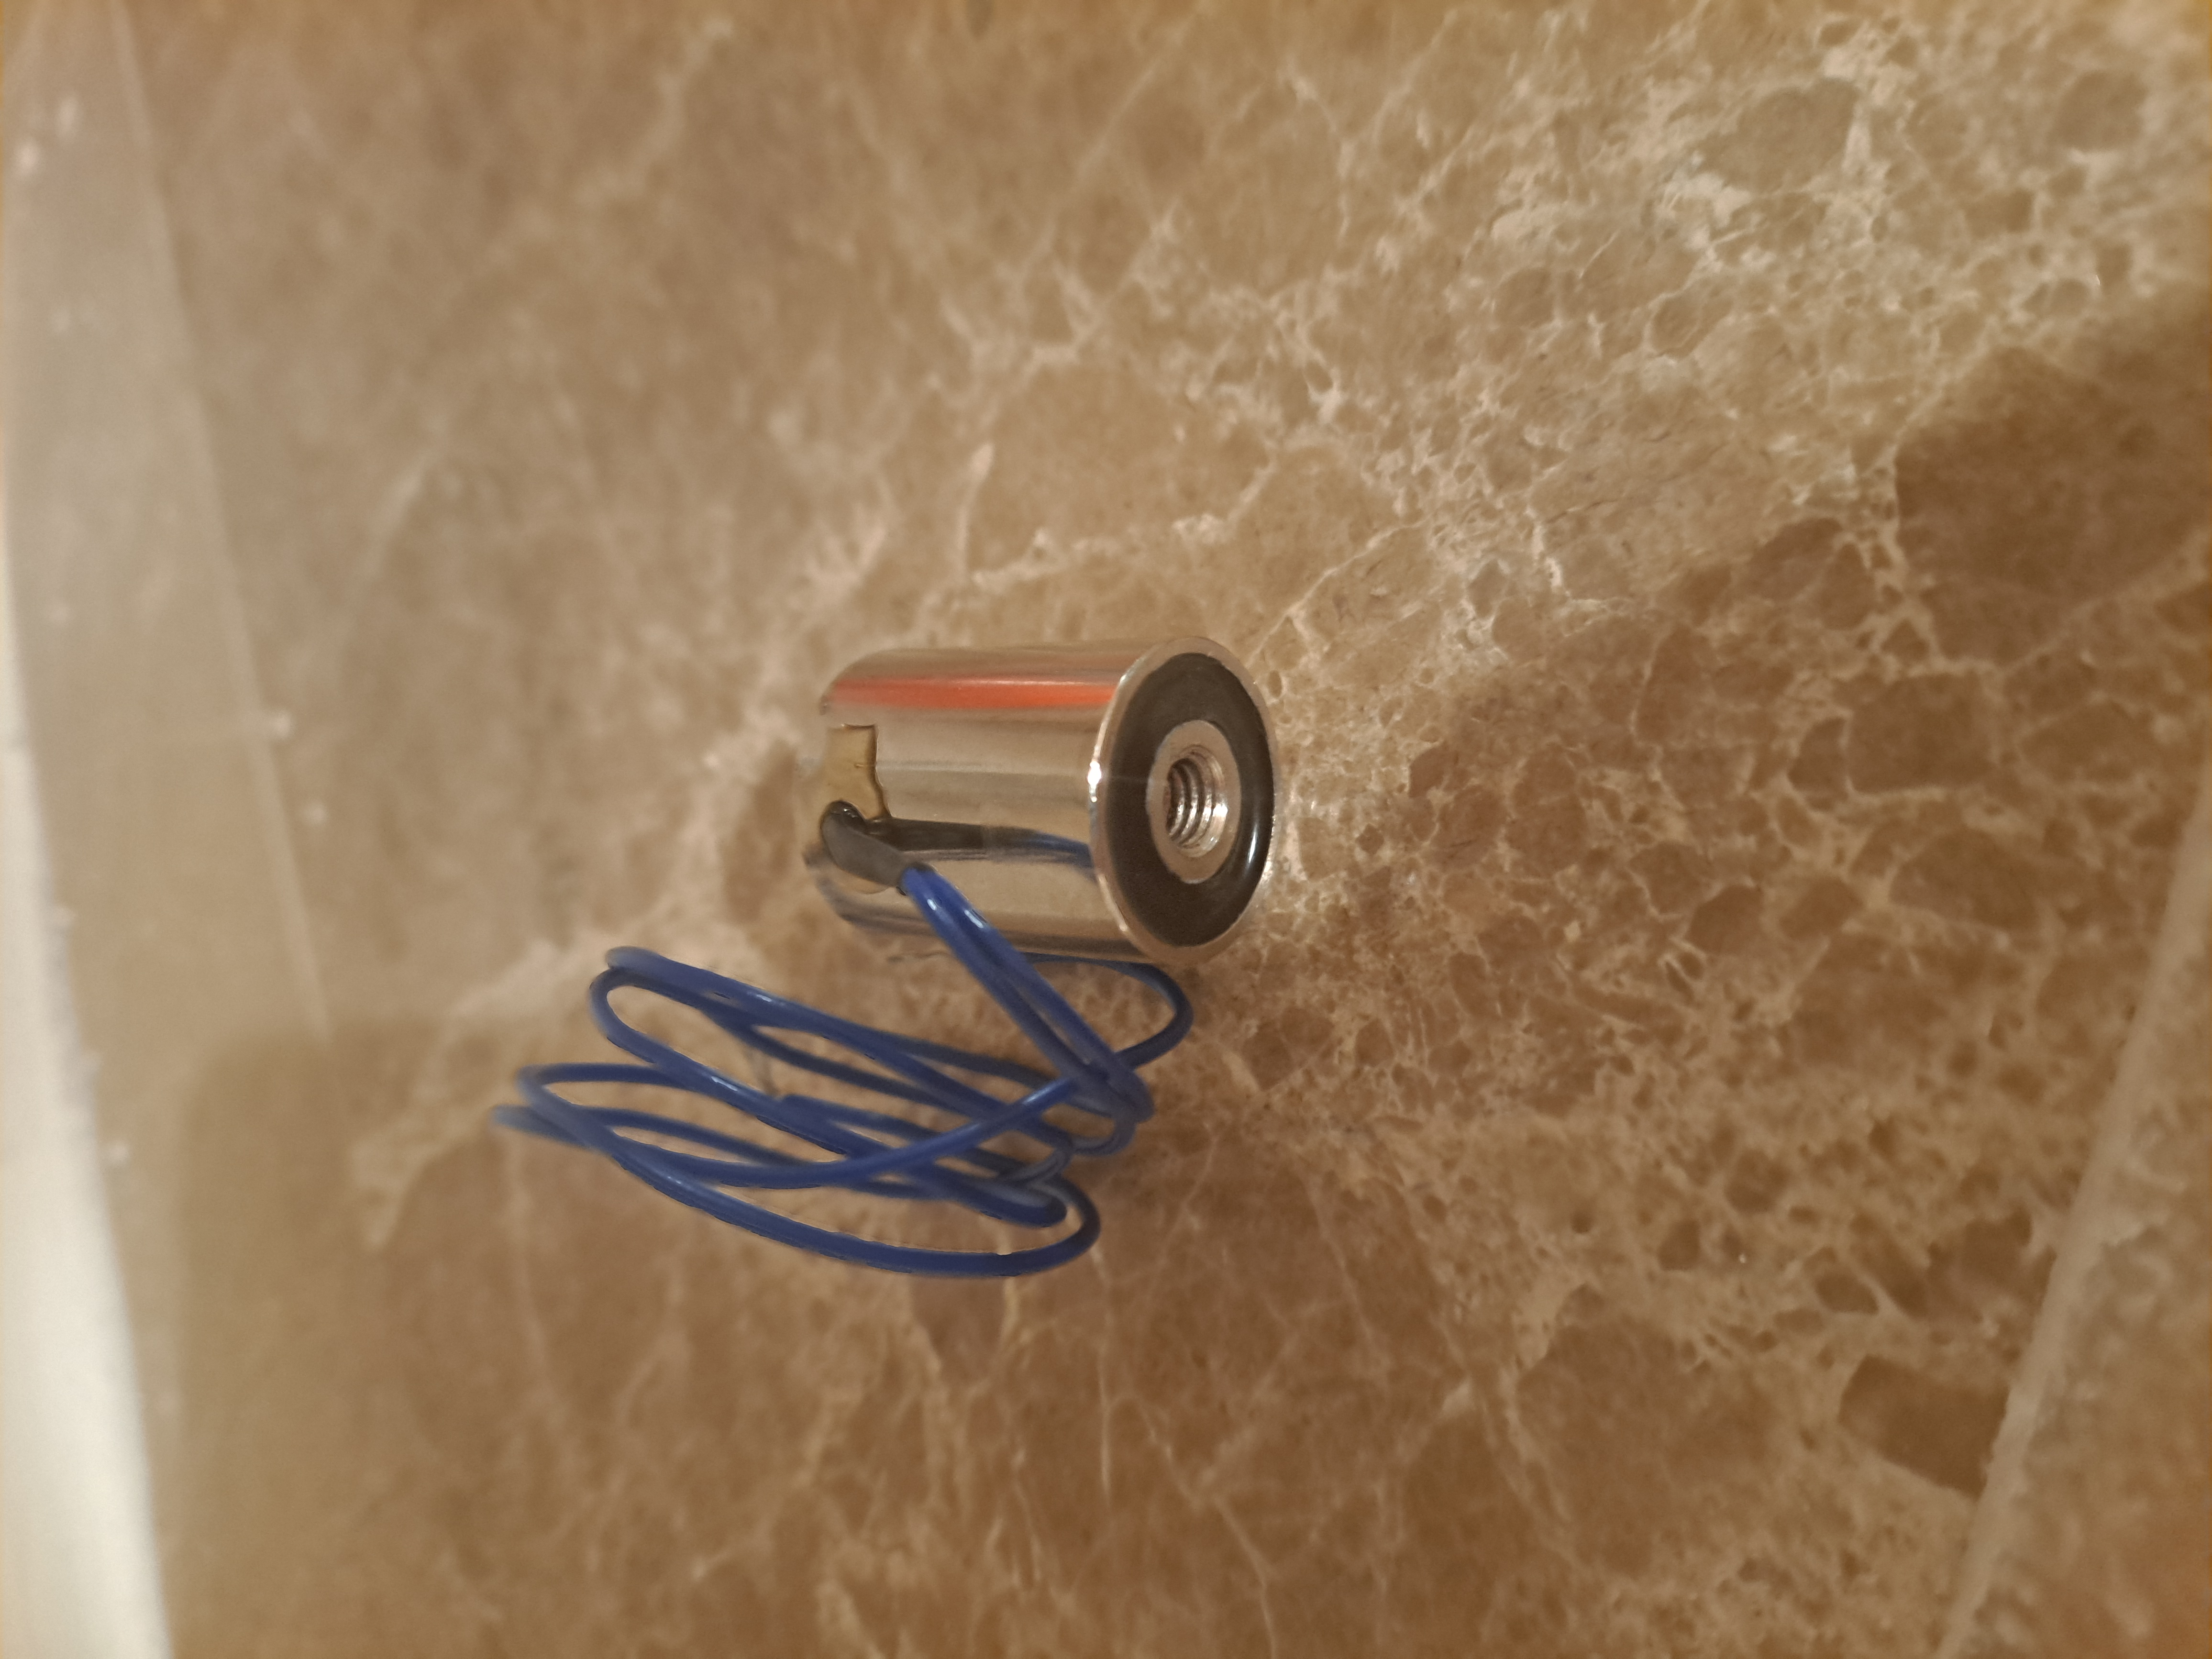
\includegraphics[width=\textwidth]{ElectromagnetImg.jpg}
    \caption{An electromagnet.}
    \label{fig:figure3}
\end{subfigure}

\caption{Three side-by-side figures showing an ESP32, a stepper motor, and an electromagnet.}
\label{fig:side_by_side}
\end{figure}
  


\subsection{Introduction to Cable-Driven Robots}

\section{Methodology}
Describe the methods or techniques used to conduct the research. Include any specific algorithms, models, or tools you implemented.
Derivation for the inverse kinematics model.
Logic behind picking constant time over constant motor velocity.
Planar Homography.


\section{Results}
Present your findings clearly using text, tables, and figures. Reference all figures and tables in the text.

\section{Discussion}
Analyze and interpret the results. Discuss their implications, limitations, and potential future work.
Could talk about why the end-effector could not be done here.
Remember to discuss the pulley problem. Using Lego connector pins as pulleys causes problems. We 3D printed pulleys
but they would slip. Limitations with the 3D printer precision.

\section{Conclusion}
Summarize the key findings and their significance. Suggest directions for further research.


\bibliographystyle{plain}
\bibliography{references}

\appendix
\section{Appendix: Additional Details}
Code snippets that are important. Instructions on how to run the project (setting up srccpy and obsstudio).

\end{document}
